\documentclass[a4paper]{article}

\usepackage[margin=1in]{geometry}

\usepackage{blindtext}
\usepackage[utf8]{inputenc}
\usepackage[greek,english]{babel}
\usepackage{alphabeta}

\usepackage{inconsolata}
\usepackage{listings}
\usepackage{xcolor}
\lstset{
    language=C, 
    basicstyle=\ttfamily\small,
    numberstyle=\footnotesize,
    numbers=left,
    backgroundcolor=\color{gray!10},
    frame=single,
    tabsize=4,
    rulecolor=\color{black!30},
    title=\lstname,
    escapeinside={\%*}{*)},
    breaklines=true,
    breakatwhitespace=true,
	showstringspaces=false,
    framextopmargin=2pt,
    framexbottommargin=2pt,
    inputencoding=utf8,
    extendedchars=true,
    literate={á}{{\'a}}1 {ã}{{\~a}}1 {é}{{\'e}}1,
}


\usepackage{graphicx}
\usepackage{subfig}
\graphicspath{ {./images/} }

\lstdefinelanguage
   [x64]{Assembler}     % add a "x64" dialect of Assembler
   [x86masm]{Assembler} % based on the "x86masm" dialect
   % with these extra keywords:
   {morekeywords={CDQE,CQO,CMPSQ,CMPXCHG16B,JRCXZ,LODSQ,MOVSXD, %
                  POPFQ,PUSHFQ,SCASQ,STOSQ,IRETQ,RDTSCP,SWAPGS, %
                  rax,rdx,rcx,rbx,rsi,rdi,rsp,rbp, %
                  r8,r8d,r8w,r8b,r9,r9d,r9w,r9b, %
                  r10,r10d,r10w,r10b,r11,r11d,r11w,r11b, %
                  r12,r12d,r12w,r12b,r13,r13d,r13w,r13b, %
                  r14,r14d,r14w,r14b,r15,r15d,r15w,r15b,
				  lw, sw, li, add, addi, csrw, lui, auipc, bgeu, 
				  bltu, jal, j, unimp, srli, andi, srai, beqz, jalr, bne,
				  bge, beq, blt, mv, xori, and, slli, or,  addi, j, srli, la,
				  .globl, .bss, .equ, .word, .space, bgt}} % etc.

\lstset{language=[x64]Assembler}

\title{ΕΘΝΙΚΟ ΜΕΤΣΟΒΙΟ ΠΟΛΥΤΕΧΝΕΙΟ\\ ~\\Αναφορά $2^{ου}$ Εργαστήριου RISC-V\\Μάθημα: Εργαστήριο Μικροϋπολογιστών}
\author{Ομάδα: Α3 \\Ονοματεπώνυμο: Μάρκος Γκέργκες\\ Αριθμός Μητρώου: 03117870}
\date{Ακαδημαϊκό Έτος 2020-21 }
\begin{document}
\maketitle

\section*{Ερώτημα 1}
\par  Tα στοιχεία των πινάκων είναι αποθηκευμένα σε συνεχόμενη μνήμη ανά 4 bytes, αφού έχουμε ορίσει σαν "τύπο" στοιχείων 
τα words (4 bytes). Αυξάνοντας έναν κατάλληλο δείκτη (διεύθυνση) κατά 4, μπορούμε να λαμβάνουμε το επόμενο στοιχείο του πίνακα.
\\Η εντολή negate(neg RegD, Reg2) χρησιμοποείται στην εύρεση της απόλυτης τιμής και έχει ως αποτέλεσμα RegD = -Reg2. Έχει την ίδια μεταγλώττιση με την SUB   RegD,x0,Reg2.
\\Μέσω του debugger-whisper, μπορούμε εφόσον θέσουμε (στον κώδικα που ακολουθεί) τον t5 στη διεύθυνση του πίνακα C, από τον πίνακα των καταχωρητών να διαβάσουμε την διεύθυνση 
που βρίσκεται στη μνήμη. Στην εικόνα που παρατίθεται βρέθηκε πως ο t5 αρχικά είχε τιμή 0x2198. Επιλέχθηκε από το πεδίο Memory να διαβαστούν 40 bytes στην διεύθυνση αυτή, δηλαδή 
10 αριθμοί. Στην τελευταία επανάληψη επιβεβαιώνεται η ορθότητα των αποτελεσμάτων που αποθηκεύονται, ενώ ο t5 έχει πλέον αυξηθεί αφού δείχνει στο τελευταίο στοιχείο του πίνακα C.

\vspace{\baselineskip}
\vspace{\baselineskip}

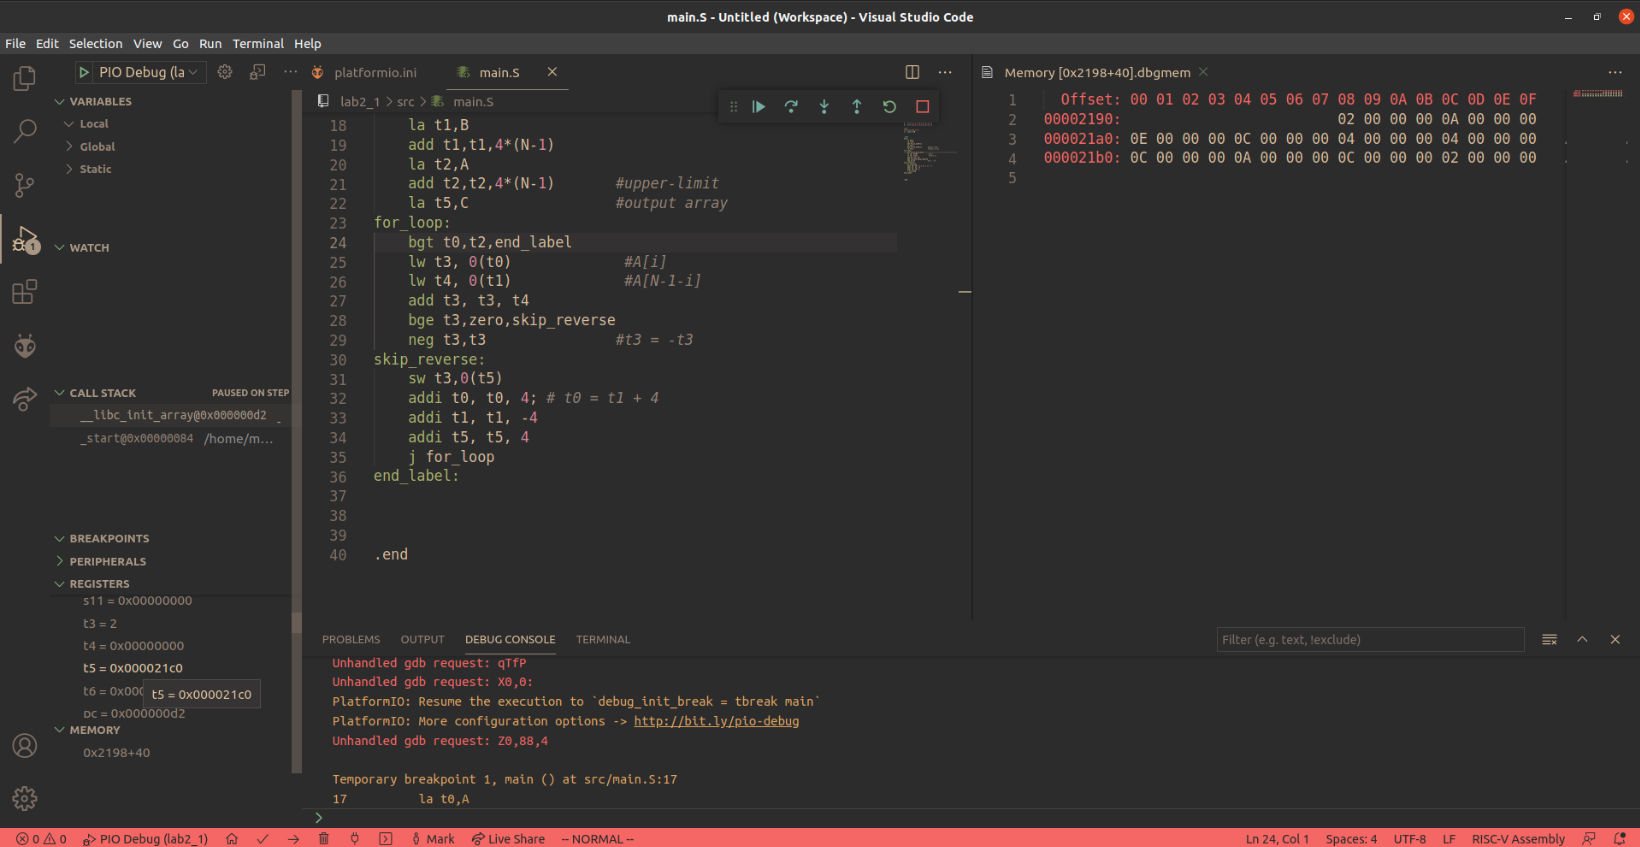
\includegraphics[width=1\linewidth]{Screenshot_riscv}

\pagebreak
\subsection*{Κώδικας Assembly}

\begin{lstlisting}[ keywordstyle=\color{red}, basicstyle=\small, extendedchars=true]
#%* με το directive .globl, μπορούμε να αναφερθούμε στην main και από άλλα αρχεία*)
.globl main 

#%* Ορίζουμε μια σταθερά, το Ν, ίση με το πλήθος των στοιχείων*)
.equ N, 10

#%* Σε αυτό το section ορίζουμε global δεδομένα που αποθηκεύονται στη μνήμη*)
.data		#%* Συγκεκριμένα πίνακες απο words, δηλαδή 4 bytes*)
A: .word 0,1,2,7,-8,4,5,-12,11,-2
B: .word 0,1,2,7,-8,4,5,12,-11,-2

.bss
#%* Σε αυτό το section μπορούμε να δεσμεύσουμε χώρο στη μνήμη, τα δεδομένα αρχικοποιούνται σε 0*)
C: .space 4*N
#%* ο C θα είναι πίνακας που χωράει 10 words*)

.text
main:
    la t0,A					#%* φορτώνουμε τη διεύθυνση του πίνακα Α*)
    la t1,B					#%* φορτώνουμε τη διεύθυνση του πίνακα Β*)
    add t1,t1,4*(N-1)		#%* αυξάνοντας την τιμή κατά 4*(Ν-1), θα δείχνει στο τελευταίο στοιχείο*)
    la t2,A					#%* θα βάλουμε σαν άνω όριο του βρόγχου τη διεύθυνση του A[N-1]*)
    add t2,t2,4*(N-1)       #%* αυξάνουμε κατά 4*(Ν-1) για να την λάβουμε*)
    la t5,C                 #%* φορτώνουμε τη διεύθυνση του πίνακα C, *) 
for_loop:					#%* όπου θα αποθηκεύσουμε τα αποτελέσματα*)
    bgt t0,t2,end_label		#%* τέλος όταν t0 δείχνει σε μεγαλύερη διέθυνση απ'το τελευταίο στοιχείο*)
    lw t3, 0(t0)            #%* φορτώνουμε το A[i] στον καταχωρητή t3*)
    lw t4, 0(t1)            #%* αντίστοιχα φορτώνουμε το Β[N-1-i] στον καταχωρητή t4 *)
    add t3, t3, t4			#%* προσθέτουμε τις 2 τιμές *) 
    bge t3,zero,skip_reverse	#%*αν είναι $\geq$0, τότε ισούται με απόλυτη τιμή *) 
    neg t3,t3               #%* αν είναι αρνητικό παίρνουμε το 2's complement με την neg*) 
skip_reverse:				
    sw t3,0(t5)				#%* αποθηκέουμε το αποτέλεσμα στον πίνακα C*) 
    addi t0, t0, 4	 	#%* αυξάνουμε τον δείκτη του πίνακα Α ώστε να δείχνει στο επόμενο στοιχείο	*) 	
    addi t1, t1, -4			#%* μειώνουμε τον δείκτη του πίνακα Β*) 
    addi t5, t5, 4			#%* αυξάνουμε τον δείκτη του πίνακα C*) 
    j for_loop				#%* συνεχίζουμε τον βρόγχο *) 
end_label:

.end
\end{lstlisting}

%-----------------------------------------------------------------------------------------------------
\vspace{\baselineskip}
\vspace{\baselineskip}
\vspace{\baselineskip}
\vspace{\baselineskip}
\vspace{\baselineskip}
\vspace{\baselineskip}
\pagebreak
\section*{Ερώτημα 2}
\par
Για να θέσουμε τα leds ως έξοδο, θέτουμε όλα τα πρώτα 16 bits της διεύθυνσης 0x80001408 ίσα με '1'. Η υλοποίηση αποτελείται από ένα διπλό βρόγχο 
που πραγματοποιεί σταδιακά την ενεργοποίηση όλων των leds, και έπειτα άλλο ένα διπλό βρόγχο που πραγματοποιεί την απενεργοποίηση τους. Οι εξωτερικοί βρόγχοι "τρέχουν" 
16 φορές, όσος και ο συνολικός αριθμός των leds, ενώ οι εσωτερικοί βρόγχοι πραγματοποιούν την ολίσθηση ενός bit, όσες φορές χρειάζεται κάθε φορά. Η κατάσταση των leds, αποτελείται από 
ένα σταθερό τμήμα bits που δεν αλλάζει, αφού έχει αλάξει σε προηγούμενη φάση, και από ένα κινητό τμήμα bits στα οποία παρατηρείται η ολίσθηση του bit (αναμμένου ή μη αντίστοιχα). 
Με τη χρήση κατάλληλης μάσκας και της εντολής AND διαχωρίζουμε τα αντίστοιχα τμήματα κάθε φορά.
\par


\subsection*{Κώδικας Assembly}

\begin{lstlisting}[ keywordstyle=\color{red}, basicstyle=\small]
.globl main

.text
main:
#GPIO_INOUT 0x80001408
#GPIO_LEDS 0x80001404---2lsB
    lui t0, 0x80001
    lui t1, 0x10    	#%* t1=0x00010000 *)
    addi t1, t1, -1 	#%* t1=0xFFFF, η τιμή που θα βάλουμε στην GPIO\_INOUT διεύθυνση *)
    sw t1, 1032(t0) 	#%* 1032 = 0x408, με offset αλλάζουμε το περιεχόμενο της διεύθυνσης 0x80001408 *)
    sw zero, 1028(t0)   #%* αρχικά όλα τα leds είναι σβηστά *)
    li s1, 15       	#%* στον s1, θα κρατάμε πόσες ολισθήσεις χρείαζεται το bit-0 κάθε φορά *)
    li s2, 0xFFFF   	#%* ψευδοεντολή που αντιστοιχεί σε lui και addi -1 *)
next_bit:
    blt s1, zero, all_on	#%* θα ολοκληρώσουμε μόλις ο s1 γίνει αρνητικός*)
    mv s3, s1       	#%* ψευδοεντολή που αντιστοιχεί σε add rd, rs, zero, κρατάμε αντίσγραφο του s1*)
    li t1, 1        	#%* σταθερά για να ανάψουμε το bit0 *)
    lw t3, 1028(t0) 	#%* φορτώνουμε στον t3 τα τρέχοντα leds  *)
    or t3, t3, t1 		#%* με χρήση της or θέτουμε το lsb = 1 *)
    sw t3, 1028(t0) 	#%* ανάβουμε τα leds που είχαμε συν το lsb*)
shift_loop:
    beq zero, s3, shift_done #%* if s3 == 0, άλμα στο shift\_done*)
    lw t3, 1028(t0)     #%* φορτώνουμε στον t3 την τιμή των leds*)
    xori t4, s2, -1     #%* παίρνουμε το One's complement του mask, αντίτοιχο της NOT *)
	and t4, t3, t4      #%* ώστε να κρατήσουμε τα leds που δεν θα ολισθηθούν*)
    and t3, t3, s2      #%* κρατάμε τα leds που θα ολισθηθούν χρησιμοποιώντας τη μάσκα (s2)*)
    slli t3, t3, 1      #%* τα ολισθαίνουμε κατά 1 bit αριστερά*)
    or t3, t4, t3       #%* συνδυάζομε την ολισθημένη τιμή με τα σταθερά leds *)
    sw t3, 1028(t0)     #%* ανάβουμε τα leds *)
    addi s3, s3, -1     #%* μειώνουμε τον μετρητή ολισθήσεων *)
    j shift_loop
    
shift_done:				#%* εδώ το bit έχει ολισθήσει μέχρι την τελική του θέση, πλέον σταθερό *)
    addi s1, s1, -1		#%* το επόμενο bit θα χρειαστεί μια ολίσθηση λιγότερη *)
    srli s2, s2, 1      #%* ενημερώνουμε την μάσκα η οποία μειώνεται κατά 1 bit *)
    j next_bit			#%* συνεχίζουμε με το επόμενο bit (θα αρχίσει από lsb) *)
all_on:
    #%* τώρα όλα τα 16 bits των leds έχουν ανάψει *) 
    li s1, 15       	#%* αντίστοιχες αρχικοποίησεις με πριν, τώρα σβήνουμε όμως*) 
    li s2, 0xFFFF   	#%* bit mask *)
next_bit_2: 
    blt s1, zero, all_off		#%* τέλος όταν ο s1(ολισθήσεις που θέλει κάθε bit) γίνει αρνητικός *)
    mv s3, s1       	#%* κρατάμε ένα αντίγραφο των ολισθήσεων που θέλει το bit(ψευδοεντολή)*)
    li t1, 0x7FFF       #%* αρχικά σβήνει το msb μόνο, σαν ψευδοεντολή γιατί η σταθερά είναι μεγάλη *)
    lw t3, 1028(t0) 	#%* φορτώνουμε την κατάσταση των leds *)
    and t3, t3, t1  	#%* κρατάμε την κατάσταση των leds σβήνωντας το msb *)
    sw t3, 1028(t0) 	#%* με αποθήκευση στη διεύθυνση των leds, τα ενημερώνουμε*)
shift_loop_2:
    beq zero, s3, shift_done_2 #%* if s3 $==$0, τότε άλμα σε shift\_done\_2*)
    lw t3, 1028(t0)     #%* αποθηκεόυμε στον t3, την κατάσταση των leds*)
    xori t4, s2, -1     #%* παίρνουμε το One's complement του mask, αντίτοιχο της NOT *)
    and t4, t3, t4      #%* κρατάμε τα leds που δεν θα ολισθηθούν*)
    srli t3, t3, 1      #%* ολισθαίνουμε κατά 1 bit δεξιά τα υπόλοιπα*)
    lui t5,0x8          #%* ανάβουμε το msb, γιατί γίνεται 0 από την δεξιά ολίσθηση*)
    or t3, t3, t5    #%* το msb θα σβήσει οριστικά από τον εξωτερικό βρόγχο, στην τελευταία επανάληψη*)
    and t3, t3, s2      #%* κόβουμε τον ls άσσο της ολίσθησης που θα επηρέαζε τα σταθερά bits [στην or]*)
    or t3, t4, t3       #%* συναδυάζουμε την ολισθημένη τιμή με τα σταθερά bits *)
    sw t3, 1028(t0)     #%* απεικονίζουμε στα leds την νέα τιμή *)
    addi s3, s3, -1     #%* μείωση του μετρητή ολίσθησης*)
    j shift_loop_2

shift_done_2:
    addi s1, s1, -1
    slli s2, s2, 1  	#%* μείωση της μάσκας κατά 1 bit από τα δεξιά *)
    lui t1, 0x10    	# t1=0x00010000
    addi t1, t1, -1 	# t1=0xFFFF
    and s2, s2, t1  	#%* σβήνουμε τον αριστερά άσσο που είναι εκτός ορίων *)
    j next_bit_2		#%* και ολοκληρώνεται η μείωση της μάσκας, μετά άλμα  *)
all_off:


.end

\end{lstlisting}



\end{document}